\section{Kiểm chứng độ bất định bằng phương pháp mô phỏng Monte Carlo}
\label{sec:4_3_monte_carlo}

Trong phân tích đo lường học thực nghiệm, ma trận hiệp phương sai (covariance matrix) thu được từ thuật toán hồi quy cung cấp một xấp xỉ tuyến tính quanh nghiệm tối ưu (local linearized estimation) đối với độ bất định của các tham số vật lý. Tuy nhiên, khi đối chiếu với các hệ thống có đặc tính phi tuyến cao hoặc khi nhiễu đầu vào không còn tuân theo mô hình đơn giản, phương pháp giải tích này có thể bộc lộ những giới hạn nhất định. Do đó, phương pháp mô phỏng Monte Carlo (Monte Carlo simulation) được ứng dụng như một công cụ mô phỏng hiệu quả nhằm kiểm tra chéo (cross-validate) mức độ lan truyền sai số thực tế trong các hệ thống xử lý dữ liệu tự động hóa.

\begin{physcore}{Cơ sở thống kê của phương pháp mô phỏng Monte Carlo}{mc_basis}
Phương pháp Monte Carlo trong đo lường học dựa trên việc thêm nhiễu ngẫu nhiên vào dữ liệu (random perturbation). Đối với các hệ thống cảm biến lấy mẫu tự động, độ bất định của biến số đầu vào (như độ phân giải thời gian và không gian) được đặc trưng bởi các phân bố chuẩn (Gaussian distributions) quanh giá trị danh định. Trong quy trình này, hàng nghìn tập dữ liệu giả lập (simulated datasets) được tạo bằng cách thêm nhiễu ngẫu nhiên vào mảng dữ liệu thực nghiệm đã được nạp từ tệp .csv. Toàn bộ tập dữ liệu giả lập sau đó được đưa vào thuật toán hồi quy để tạo ra một phân bố thống kê (statistical distribution) đối với tham số vật lý cần ước lượng (trong bài toán minh họa là gia tốc trọng trường $g$). Các đại lượng thống kê (cụ thể là độ lệch chuẩn) được rút ra từ phân bố này sẽ được dùng làm độ bất định tổng thể của toàn bộ phép đo.
\end{physcore}

Quá trình giả lập dữ liệu tại từng vòng lặp được mô tả bằng phép cộng tuyến tính giữa tín hiệu thực tế và thành phần nhiễu.

\begin{derivation}{Mô hình toán học của nhiễu ngẫu nhiên}{mc_perturbation_model}
Tại vòng lặp thứ $k$, tập dữ liệu tọa độ $s_{\text{sim}}$ và thời gian $t_{\text{sim}}$ được tái tạo bằng cách cộng thêm nhiễu phân bố chuẩn vào tập dữ liệu gốc:
\begin{align}
    s_{\text{sim}, i} &= s_i + \mathcal{N}(0, \sigma_s^2) \\
    t_{\text{sim}, i} &= t_i + \mathcal{N}(0, \sigma_t^2)
\end{align}
Trong đó, $\mathcal{N}(0, \sigma^2)$ là hàm sinh số giả ngẫu nhiên tuân theo phân bố chuẩn có giá trị trung bình bằng $0$ và phương sai tương ứng với bình phương giới hạn độ phân giải của thiết bị đo. Đối với mỗi cặp mảng dữ liệu giả lập thu được, hàm mục tiêu bình phương tối thiểu được tối ưu hóa lại để xác định một giá trị ước lượng $g_{\text{mc}}^{(k)}$.
\end{derivation}

Đoạn mã dưới đây tự động hóa quy trình phân tích Monte Carlo đối với hằng số gia tốc rơi tự do.

\begin{pycode}{Monte Carlo simulation for parameter uncertainty}
import numpy as np
import matplotlib.pyplot as plt
from scipy.optimize import curve_fit

# 3. Monte Carlo Simulation for Parameter Uncertainty (Gravitational Acceleration)
num_simulations = 5000
np.random.seed(42)

g_mc_results = np.zeros(num_simulations)

for i in range(num_simulations):
    # Inject Gaussian noise strictly aligned with instrumental uncertainties
    s_simulated = displacement_data + np.random.normal(0, sigma_s, len(displacement_data))
    t_simulated = time_data + np.random.normal(0, sigma_t, len(time_data))
    
    try:
        popt_mc, _ = curve_fit(
            quadratic_displacement_model,
            t_simulated,
            s_simulated,
            p0=[9.8, 0.0, 0.0],
            maxfev=2000
        )
        g_mc_results[i] = popt_mc[0]
    except RuntimeError:
        g_mc_results[i] = np.nan

# Compute statistical limits from valid inferences
g_mc_clean = g_mc_results[~np.isnan(g_mc_results)]
g_mean = np.mean(g_mc_clean)
g_std = np.std(g_mc_clean)

# Histogram Visualization of State Space
fig_mc, ax_mc = plt.subplots(figsize=(8, 5))
ax_mc.hist(g_mc_clean, bins=50, density=True, color='steelblue', edgecolor='black', alpha=0.7)
ax_mc.axvline(g_mean, color='red', linestyle='-', linewidth=2, label=fr'$\mathrm{{Mean}}: {g_mean:.3f} \ \mathrm{{m/s^2}}$')
ax_mc.axvline(g_mean + g_std, color='darkorange', linestyle='--', linewidth=2, label=r'$+1 \ \mathrm{Std \ Dev}$')
ax_mc.axvline(g_mean - g_std, color='darkorange', linestyle='--', linewidth=2, label=r'$-1 \ \mathrm{Std \ Dev}$')

ax_mc.set_title(r'$\mathrm{Monte \ Carlo \ Inference: \ Gravitational \ Acceleration}$')
ax_mc.set_xlabel(r'$\mathrm{Parameter \ Space} \ g \ (\mathrm{m/s^2})$')
ax_mc.set_ylabel(r'$\mathrm{Probability \ Density}$')
ax_mc.legend()
ax_mc.grid(True, linestyle=':', alpha=0.6)
plt.show()

print(f"Monte Carlo Inference Result: g = {g_mean:.4f} +/- {g_std:.4f} m/s^2")
\end{pycode}

\begin{figure}[htbp]
    \centering
    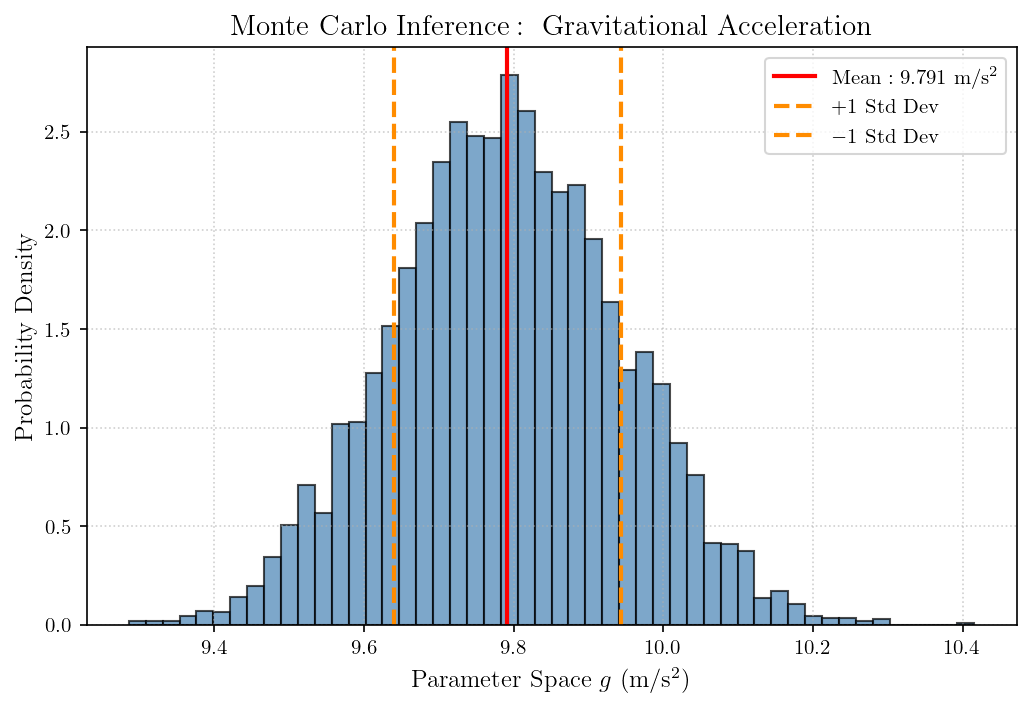
\includegraphics[width=\textwidth]{figures/fig_monte_carlo_hist.png}
    \caption{Phân bố của giá trị gia tốc trọng trường thu được thông qua mô phỏng Monte Carlo.}
    \label{fig:monte_carlo_hist}
\end{figure}

Biểu đồ tần suất (histogram) thu được cho thấy xu hướng tiến gần phân bố chuẩn của tham số gia tốc. Độ lệch chuẩn trích xuất từ mảng giá trị hợp lệ (\texttt{g\_mc\_clean}) được dùng để ước lượng độ bất định tổng thể cho kết quả hồi quy.

% \begin{pitfall}{Rủi ro phân kỳ thuật toán và dao động thống kê}{mc_algorithm_risk}
\begin{pitfall}{Sự phân kỳ thuật toán và nhiễu thống kê do cỡ mẫu nhỏ}{mc_algorithm_risk}
Độ ổn định của kết quả ước lượng từ mô phỏng Monte Carlo phụ thuộc chặt chẽ vào kích thước mẫu (\texttt{num\_simulations}). Số lượng vòng lặp quá nhỏ dễ gây ra các dao động thống kê, làm ảnh hưởng đến độ tin cậy của độ lệch chuẩn được tính toán. Hơn nữa, việc thêm nhiễu ngẫu nhiên trực tiếp vào mảng dữ liệu có khả năng sinh ra các giá trị không phù hợp về mặt vật lý (ví dụ: vật thể di chuyển lùi trong một bước thời gian cực ngắn do sai số giả lập lớn). Những điểm dữ liệu dị biệt này có thể khiến thuật toán lặp (như Levenberg-Marquardt) từ chối hội tụ, dẫn đến việc phát sinh ngoại lệ \texttt{RuntimeError}. Để quá trình mô phỏng ổn định hơn, ta cần đặt hàm \texttt{curve\_fit} trong khối lệnh \texttt{try...except} nhằm xử lý lỗi phân kỳ và gán giá trị rỗng (\texttt{np.nan}) cho kết quả thất bại. Cách xử lý này cho phép thuật toán dễ dàng thanh lọc dữ liệu dị biệt (thông qua hàm \texttt{\textasciitilde np.isnan}) trước khi trích xuất thống kê cuối cùng. Ngoài ra, việc thiết lập hạt giống khởi tạo bằng hàm \texttt{np.random.seed} là yêu cầu thiết yếu để đảm bảo khả năng tái lập (reproducibility) của phép tính.
\end{pitfall}

Sự tương đồng giữa độ bất định thu được từ mô phỏng Monte Carlo (\texttt{g\_std}) và độ bất định trích xuất trực tiếp từ cấu trúc ma trận hiệp phương sai (\texttt{g\_s\_err}) cho thấy mô hình hồi quy hoạt động ổn định. Mối tương quan này cho thấy các giới hạn phân giải của thiết bị đo đã được phản ánh nhất quán trong toàn bộ quá trình tính toán của bài toán động học.